% report/figures_preview.tex - compiles every figure on its own pages,
% so the figures can be checked without building the whole report.
%   pdflatex figures_preview.tex
\documentclass[11pt,a4paper]{article}
\usepackage[margin=2.5cm]{geometry}
\usepackage{amsmath,amssymb}
\usepackage{tikz}
\usetikzlibrary{positioning,arrows.meta,shapes,fit,calc,backgrounds}
\usepackage{pgfplots}
\pgfplotsset{compat=1.18}
% report/figures/styles.tex - shared TikZ styles for every diagram.
% Needs: \usepackage{tikz} and \usetikzlibrary{positioning,arrows.meta,shapes,fit,calc,backgrounds}
%
% Colour encodes the role of a box, using the validated categorical palette:
% grey for data, blue for knowledge, orange for reasoning, aqua for outputs.
% Every box also carries a text label, so colour is never the only cue.

\definecolor{inkMain}{HTML}{262624}
\definecolor{inkSoft}{HTML}{6B6A64}
\definecolor{accBlue}{HTML}{2A78D6}
\definecolor{accOrange}{HTML}{EB6834}
\definecolor{accAqua}{HTML}{1BAF7A}

\tikzset{
  base/.style={draw=inkSoft, line width=0.5pt, rounded corners=2pt, align=center,
               font=\small, text=inkMain, inner sep=3pt, minimum height=8mm},
  box/.style={base, text width=#1},
  box/.default=3cm,
  data/.style={box=#1, fill=black!5},
  data/.default=3cm,
  kb/.style={box=#1, fill=accBlue!10, draw=accBlue!80!black},
  kb/.default=3cm,
  reason/.style={box=#1, fill=accOrange!10, draw=accOrange!85!black},
  reason/.default=3cm,
  out/.style={box=#1, fill=accAqua!12, draw=accAqua!80!black},
  out/.default=3cm,
  ext/.style={box=#1, fill=white, dashed},
  ext/.default=3cm,
  decision/.style={diamond, aspect=2.2, draw=accOrange!85!black, fill=accOrange!6,
                   line width=0.5pt, align=center, font=\footnotesize, text=inkMain,
                   inner sep=1pt, text width=#1},
  decision/.default=2.6cm,
  flow/.style={-{Stealth[length=2mm,width=1.6mm]}, draw=inkSoft, line width=0.6pt},
  uses/.style={flow, dashed},
  feedback/.style={flow, dashed, draw=accOrange!85!black},
  air/.style={-{Stealth[length=2.2mm,width=1.8mm]}, line width=1.1pt},
  cold/.style={air, draw=accBlue},
  hot/.style={air, draw=accOrange},
  water/.style={-{Stealth[length=1.8mm]}, line width=0.8pt, draw=accBlue!70!black},
  power/.style={line width=0.9pt, draw=inkMain},
  note/.style={font=\footnotesize\itshape, text=inkSoft, align=center},
  tag/.style={font=\scriptsize, text=inkSoft},
  group/.style={draw=inkSoft, dashed, rounded corners=3pt, inner sep=5pt},
  grouplabel/.style={font=\footnotesize\bfseries, text=inkSoft},
  sensor/.style={circle, draw=accBlue!80!black, fill=white, line width=0.5pt,
                 inner sep=0pt, minimum size=3.6mm, font=\scriptsize\bfseries, text=accBlue!80!black},
}

\begin{document}
\section*{fig\_system\_schematic}
\begin{center}
% Figure 1: industrial system schematic (plan view of the row).
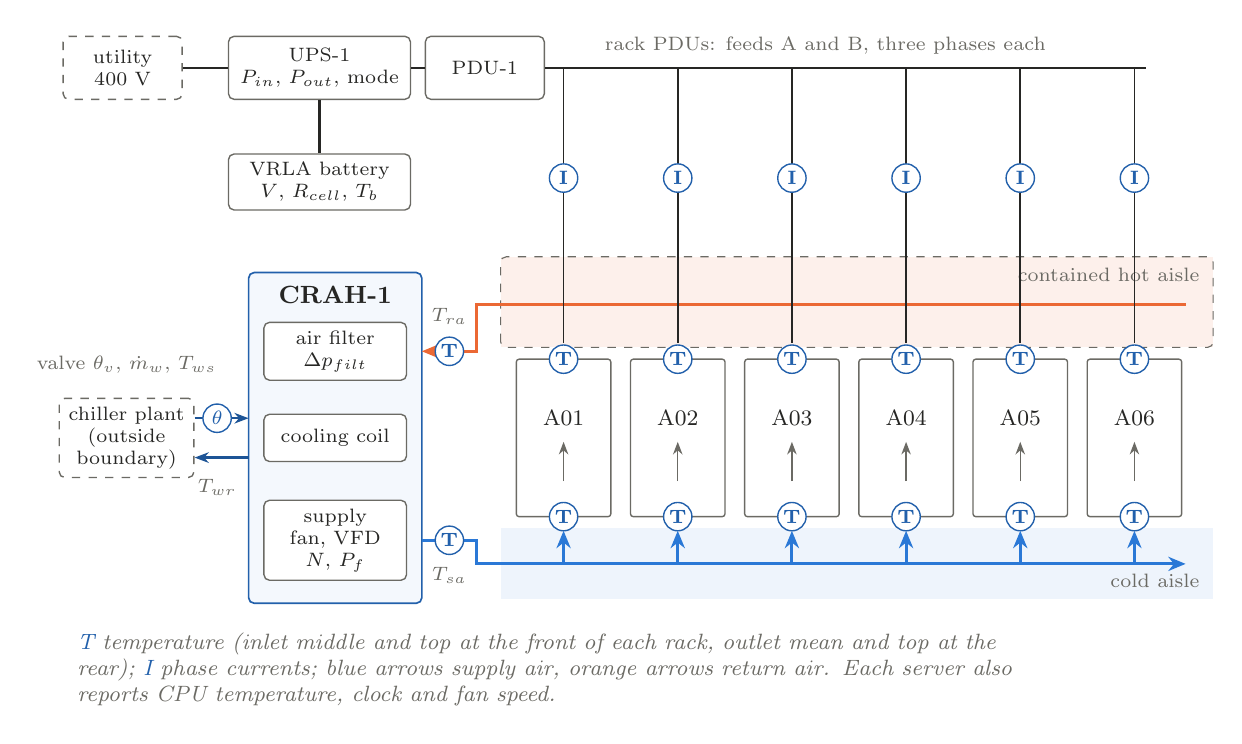
\begin{tikzpicture}[x=1cm, y=1cm]
  % ---- aisles (drawn first so everything else sits on top)
  \fill[accBlue!8] (3.2,0.25) rectangle (12.25,1.15);
  \fill[accOrange!10] (3.2,3.45) rectangle (12.25,4.6);
  \draw[inkSoft, dashed, rounded corners=2pt] (3.2,3.45) rectangle (12.25,4.6);
  \node[tag, anchor=south east] at (12.2,0.27) {cold aisle};
  \node[tag, anchor=north east] at (12.2,4.58) {contained hot aisle};

  % ---- racks
  \foreach \i in {1,...,6} {
    \pgfmathsetmacro{\xa}{3.4 + (\i-1)*1.45}
    \pgfmathsetmacro{\xc}{\xa + 0.6}
    \draw[inkSoft, fill=white, line width=0.5pt, rounded corners=1pt] (\xa,1.3) rectangle ++(1.2,2.0);
    \node[font=\footnotesize, text=inkMain] at (\xc,2.55) {A0\i};
    \draw[-{Stealth[length=1.6mm]}, draw=inkSoft, line width=0.5pt] (\xc,1.75) -- (\xc,2.25);
    \node[sensor] at (\xc,1.3) {T};
    \node[sensor] at (\xc,3.3) {T};
    \draw[cold] (\xc,0.7) -- (\xc,1.12);
  }

  % ---- cooling unit
  \draw[accBlue!80!black, fill=accBlue!5, line width=0.6pt, rounded corners=2pt] (0,0.2) rectangle (2.2,4.4);
  \node[font=\small\bfseries, text=inkMain] at (1.1,4.12) {CRAH-1};
  \node[base, fill=white, text width=1.6cm, font=\scriptsize, minimum height=6mm] at (1.1,3.4) {air filter\\ $\Delta p_{filt}$};
  \node[base, fill=white, text width=1.6cm, font=\scriptsize, minimum height=6mm] at (1.1,2.3) {cooling coil};
  \node[base, fill=white, text width=1.6cm, font=\scriptsize, minimum height=6mm] at (1.1,1.0) {supply fan, VFD\\ $N$, $P_f$};

  % ---- air paths
  \draw[cold] (2.2,1.0) -- (2.9,1.0) |- (11.9,0.7);
  \draw[hot] (11.9,4.0) -- (2.9,4.0) |- (2.2,3.4);
  \node[sensor] at (2.55,1.0) {T};
  \node[tag, anchor=north] at (2.55,0.78) {$T_{sa}$};
  \node[sensor] at (2.55,3.4) {T};
  \node[tag, anchor=south] at (2.55,3.62) {$T_{ra}$};

  % ---- chilled water
  \node[ext=1.5cm, font=\scriptsize] (plant) at (-1.55,2.3) {chiller plant\\ (outside\\ boundary)};
  \draw[water] (plant.east |- 0,2.55) -- (0,2.55);
  \draw[water] (0,2.05) -- (plant.east |- 0,2.05);
  \node[sensor] at (-0.4,2.55) {$\theta$};
  \node[tag, anchor=south] at (-1.55,3.0) {valve $\theta_v$, $\dot m_w$, $T_{ws}$};
  \node[tag, anchor=north] at (-0.4,1.9) {$T_{wr}$};

  % ---- power path
  \node[ext=1.3cm, font=\scriptsize] (util) at (-1.6,7.0) {utility\\ 400 V};
  \node[base, fill=white, text width=2.1cm, font=\scriptsize] (ups) at (0.9,7.0) {UPS-1\\ $P_{in}$, $P_{out}$, mode};
  \node[base, fill=white, text width=2.1cm, font=\scriptsize, minimum height=6mm] (bat) at (0.9,5.55) {VRLA battery\\ $V$, $R_{cell}$, $T_b$};
  \node[base, fill=white, text width=1.3cm, font=\scriptsize] (pdu) at (3.0,7.0) {PDU-1};
  \draw[power] (util) -- (ups);
  \draw[power] (ups) -- (pdu);
  \draw[power] (ups) -- (bat);
  \draw[power] (pdu.east) -- (11.4,7.0);
  \foreach \i in {1,...,6} {
    \pgfmathsetmacro{\xc}{3.4 + (\i-1)*1.45 + 0.6}
    \draw[power, line width=0.6pt] (\xc,7.0) -- (\xc,3.5);
    \node[sensor] at (\xc,5.6) {I};
  }
  \node[tag, anchor=south west] at (4.4,7.05) {rack PDUs: feeds A and B, three phases each};

  % ---- key
  \node[note, anchor=north west, text width=12cm, align=left] at (-2.3,-0.05)
    {\textcolor{accBlue!80!black}{T}~temperature (inlet middle and top at the front of each rack, outlet mean and top at the rear);
     \textcolor{accBlue!80!black}{I}~phase currents; blue arrows supply air, orange arrows return air.
     Each server also reports CPU temperature, clock and fan speed.};
\end{tikzpicture}

\end{center}
\clearpage
\section*{fig\_architecture}
\begin{center}
% Figure 2: expert-system architecture.
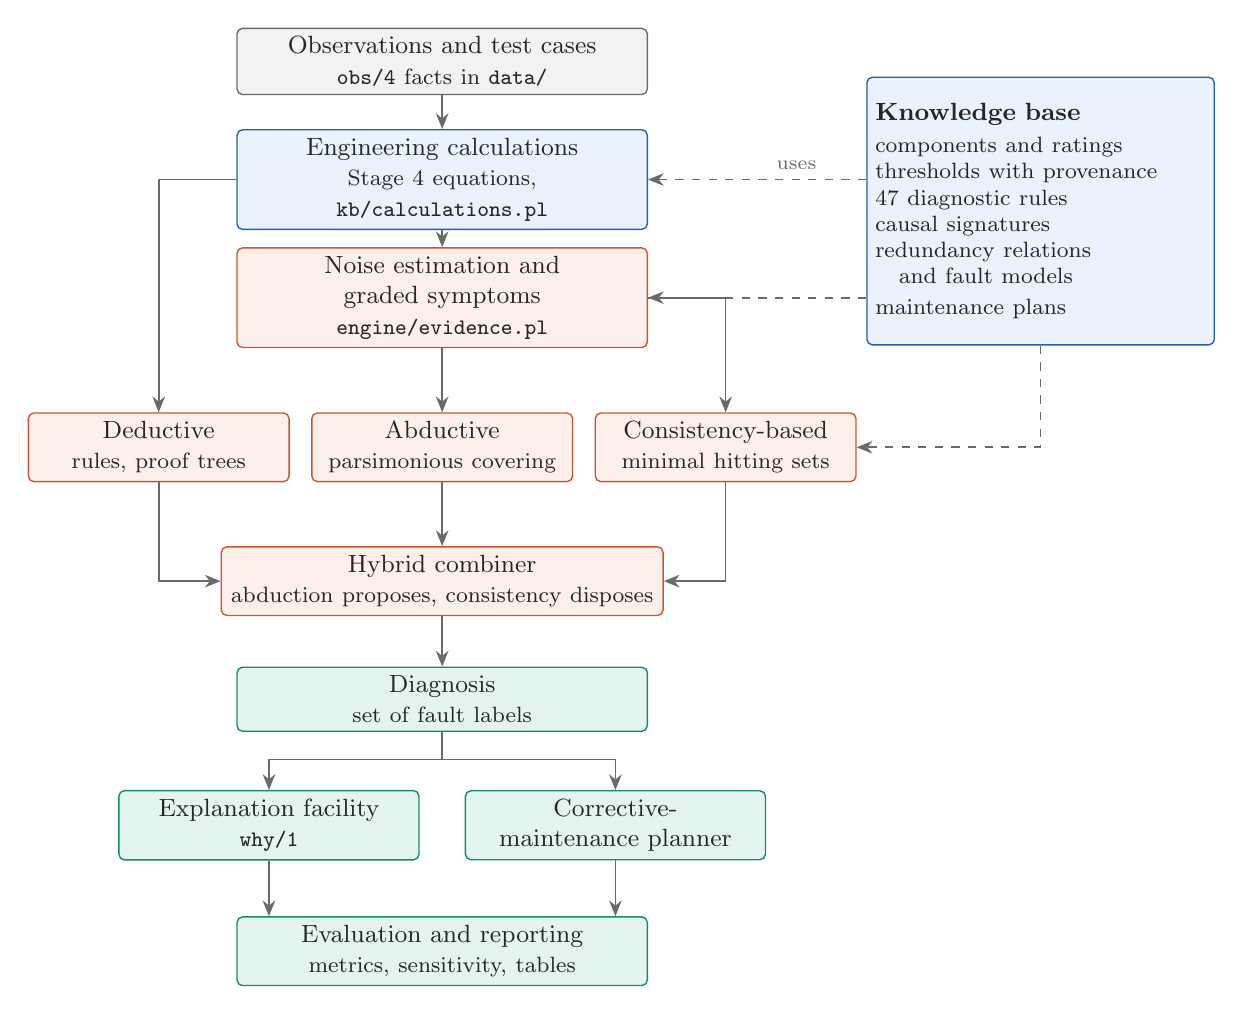
\begin{tikzpicture}[x=1cm, y=1cm]
  \node[data=5cm] (obs) at (4.5,0) {Observations and test cases\\ \footnotesize\texttt{obs/4} facts in \texttt{data/}};
  \node[kb=5cm] (calc) at (4.5,-1.5) {Engineering calculations\\ \footnotesize Stage 4 equations, \texttt{kb/calculations.pl}};
  \node[reason=5cm] (evid) at (4.5,-3.0) {Noise estimation and graded symptoms\\ \footnotesize \texttt{engine/evidence.pl}};

  \node[kb=4.2cm, minimum height=3.4cm, align=left] (kb) at (12.1,-1.9)
    {\textbf{Knowledge base}\\[2pt]
     \footnotesize components and ratings\\
     \footnotesize thresholds with provenance\\
     \footnotesize 47 diagnostic rules\\
     \footnotesize causal signatures\\
     \footnotesize redundancy relations\\
     \footnotesize \quad and fault models\\
     \footnotesize maintenance plans};

  \node[reason=3.1cm] (ded) at (0.9,-4.9) {Deductive\\ \footnotesize rules, proof trees};
  \node[reason=3.1cm] (abd) at (4.5,-4.9) {Abductive\\ \footnotesize parsimonious covering};
  \node[reason=3.1cm] (cbd) at (8.1,-4.9) {Consistency-based\\ \footnotesize minimal hitting sets};

  \node[reason=5.4cm] (hyb) at (4.5,-6.6) {Hybrid combiner\\ \footnotesize abduction proposes, consistency disposes};
  \node[out=5cm] (diag) at (4.5,-8.1) {Diagnosis\\ \footnotesize set of fault labels};
  \node[out=3.6cm] (expl) at (2.3,-9.7) {Explanation facility\\ \footnotesize \texttt{why/1}};
  \node[out=3.6cm] (maint) at (6.7,-9.7) {Corrective-maintenance planner};
  \node[out=5cm] (eval) at (4.5,-11.3) {Evaluation and reporting\\ \footnotesize metrics, sensitivity, tables};

  \draw[flow] (obs) -- (calc);
  \draw[flow] (calc) -- (evid);
  \draw[flow] (calc.west) -| (ded.north);
  \draw[flow] (evid) -- (abd);
  \draw[flow] (evid.east) -| (cbd.north);
  \draw[flow] (ded.south) |- (hyb.west);
  \draw[flow] (abd) -- (hyb);
  \draw[flow] (cbd.south) |- (hyb.east);
  \draw[flow] (hyb) -- (diag);
  \draw[flow] (diag.south) -- ++(0,-0.35) -| (expl.north);
  \draw[flow] (diag.south) -- ++(0,-0.35) -| (maint.north);
  \draw[flow] (expl.south) -- (expl.south |- eval.north);
  \draw[flow] (maint.south) -- (maint.south |- eval.north);

  \draw[uses] (kb.west |- calc.east) -- (calc.east);
  \draw[uses] (kb.west |- evid.east) -- (evid.east);
  \draw[uses] (kb.south) |- (cbd.east);
  \node[tag, anchor=south] at (9.0,-1.5) {uses};
\end{tikzpicture}

\end{center}
\clearpage
\section*{fig\_knowledge\_acquisition}
\begin{center}
% Figure 3: knowledge-acquisition workflow.
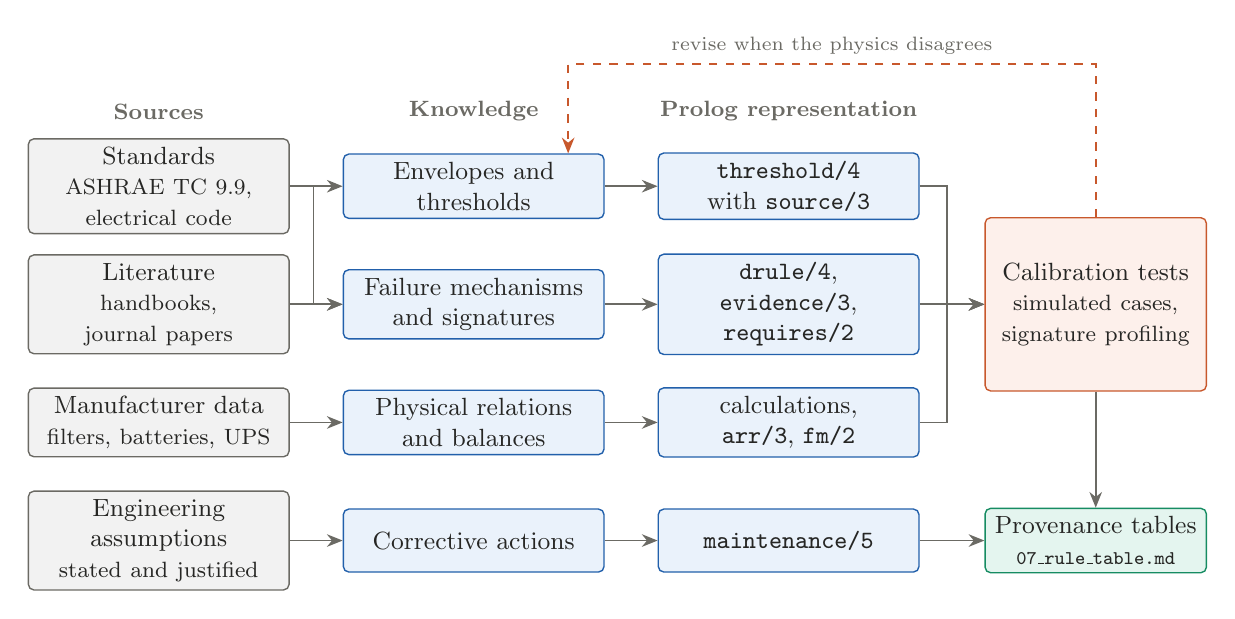
\begin{tikzpicture}[x=1cm, y=1cm]
  \node[grouplabel] at (1.6,0.95) {Sources};
  \node[data=3.1cm] (s1) at (1.6,0) {Standards\\ \footnotesize ASHRAE TC 9.9, electrical code};
  \node[data=3.1cm] (s2) at (1.6,-1.5) {Literature\\ \footnotesize handbooks, journal papers};
  \node[data=3.1cm] (s3) at (1.6,-3.0) {Manufacturer data\\ \footnotesize filters, batteries, UPS};
  \node[data=3.1cm] (s4) at (1.6,-4.5) {Engineering assumptions\\ \footnotesize stated and justified};

  \node[grouplabel] at (5.6,0.95) {Knowledge};
  \node[kb=3.1cm] (k1) at (5.6,0) {Envelopes and thresholds};
  \node[kb=3.1cm] (k2) at (5.6,-1.5) {Failure mechanisms and signatures};
  \node[kb=3.1cm] (k3) at (5.6,-3.0) {Physical relations and balances};
  \node[kb=3.1cm] (k4) at (5.6,-4.5) {Corrective actions};

  \node[grouplabel] at (9.6,0.95) {Prolog representation};
  \node[kb=3.1cm] (r1) at (9.6,0) {\texttt{threshold/4}\\ with \texttt{source/3}};
  \node[kb=3.1cm] (r2) at (9.6,-1.5) {\texttt{drule/4}, \texttt{evidence/3}, \texttt{requires/2}};
  \node[kb=3.1cm] (r3) at (9.6,-3.0) {calculations, \texttt{arr/3}, \texttt{fm/2}};
  \node[kb=3.1cm] (r4) at (9.6,-4.5) {\texttt{maintenance/5}};

  \node[reason=2.6cm, minimum height=2.2cm] (test) at (13.5,-1.5) {Calibration tests\\ \footnotesize simulated cases, signature profiling};
  \node[out=2.6cm] (table) at (13.5,-4.5) {Provenance tables\\ \scriptsize \texttt{07\_rule\_table.md}};

  \foreach \i in {1,2,3,4} { \draw[flow] (s\i) -- (k\i); \draw[flow] (k\i) -- (r\i); }
  \draw[flow] (s1.east) -- ++(0.3,0) |- (k2.west);
  \draw[flow] (r1.east) -- ++(0.35,0) |- (test.west);
  \draw[flow] (r2.east) -- (test.west |- r2.east);
  \draw[flow] (r3.east) -- ++(0.35,0) |- (test.west);
  \draw[flow] (r4) -- (table);
  \draw[flow] (test) -- (table);
  \draw[feedback] (test.north) -- (13.5,1.55) -- node[tag, above] {revise when the physics disagrees} (6.8,1.55) -- (k1.north -| 6.8,0);
\end{tikzpicture}

\end{center}
\clearpage
\section*{fig\_fault\_propagation}
\begin{center}
% Figure 4: fault propagation and causal structure.
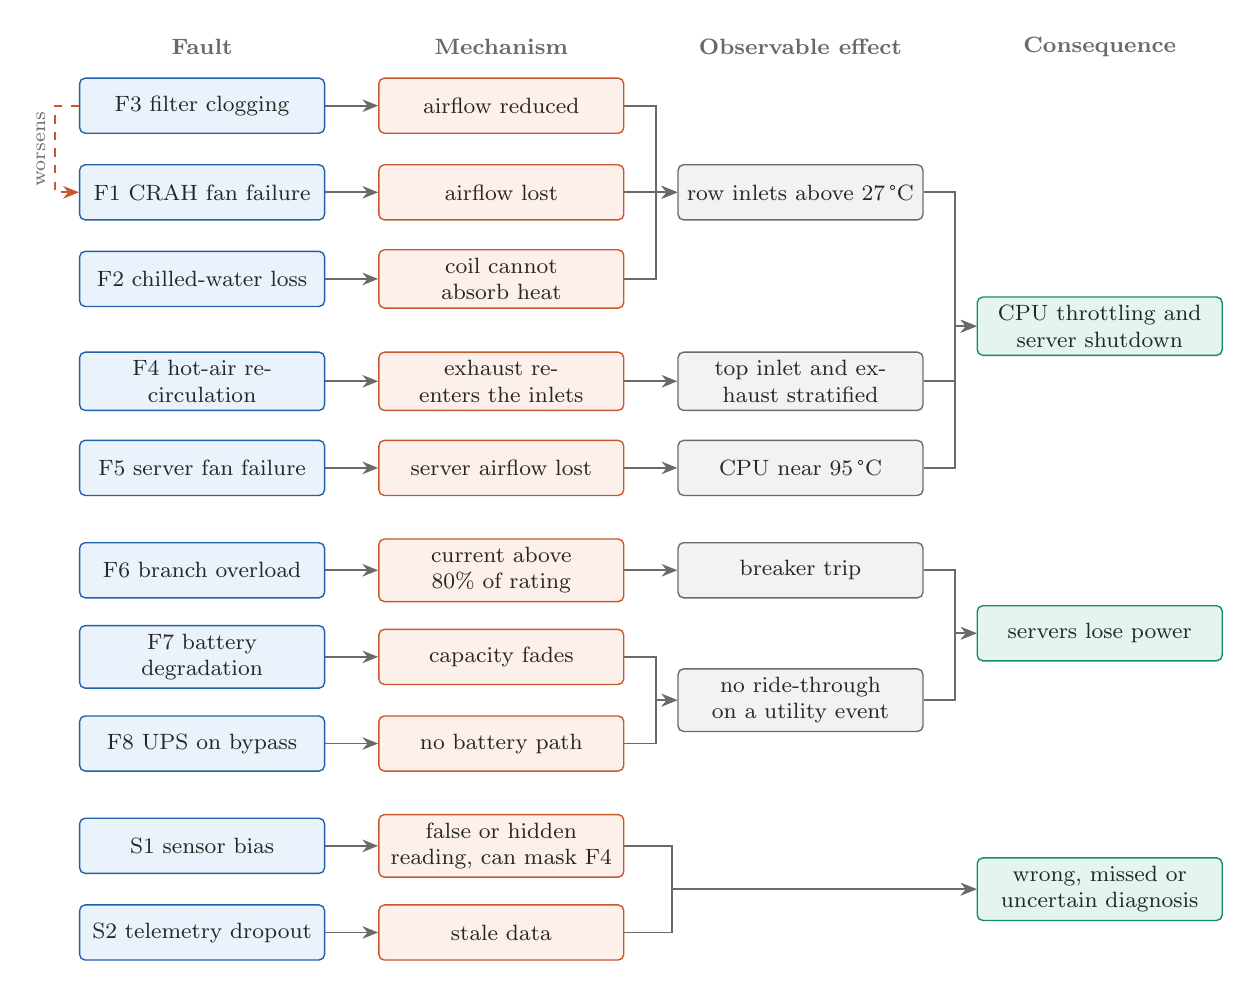
\begin{tikzpicture}[x=1cm, y=1cm]
  \node[grouplabel] at (1.5,0.75) {Fault};
  \node[grouplabel] at (5.3,0.75) {Mechanism};
  \node[grouplabel] at (9.1,0.75) {Observable effect};
  \node[grouplabel] at (12.9,0.75) {Consequence};

  \tikzset{f/.style={kb=2.9cm, font=\footnotesize, minimum height=7mm},
           m/.style={reason=2.9cm, font=\footnotesize, minimum height=7mm},
           e/.style={data=2.9cm, font=\footnotesize, minimum height=7mm},
           c/.style={out=2.9cm, font=\footnotesize, minimum height=7mm}}

  % cooling chain
  \node[f] (f3) at (1.5,0)    {F3 filter clogging};
  \node[f] (f1) at (1.5,-1.1) {F1 CRAH fan failure};
  \node[f] (f2) at (1.5,-2.2) {F2 chilled-water loss};
  \node[m] (m3) at (5.3,0)    {airflow reduced};
  \node[m] (m1) at (5.3,-1.1) {airflow lost};
  \node[m] (m2) at (5.3,-2.2) {coil cannot absorb heat};
  \node[e] (e1) at (9.1,-1.1) {row inlets above 27\,\textdegree C};
  % rack and server
  \node[f] (f4) at (1.5,-3.5) {F4 hot-air recirculation};
  \node[m] (m4) at (5.3,-3.5) {exhaust re-enters the inlets};
  \node[e] (e4) at (9.1,-3.5) {top inlet and exhaust stratified};
  \node[f] (f5) at (1.5,-4.6) {F5 server fan failure};
  \node[m] (m5) at (5.3,-4.6) {server airflow lost};
  \node[e] (e5) at (9.1,-4.6) {CPU near 95\,\textdegree C};
  \node[c] (c1) at (12.9,-2.8) {CPU throttling and server shutdown};
  % power
  \node[f] (f6) at (1.5,-5.9) {F6 branch overload};
  \node[m] (m6) at (5.3,-5.9) {current above 80\% of rating};
  \node[e] (e6) at (9.1,-5.9) {breaker trip};
  \node[f] (f7) at (1.5,-7.0) {F7 battery degradation};
  \node[m] (m7) at (5.3,-7.0) {capacity fades};
  \node[f] (f8) at (1.5,-8.1) {F8 UPS on bypass};
  \node[m] (m8) at (5.3,-8.1) {no battery path};
  \node[e] (e7) at (9.1,-7.55) {no ride-through on a utility event};
  \node[c] (c2) at (12.9,-6.7) {servers lose power};
  % instrumentation
  \node[f] (s1) at (1.5,-9.4) {S1 sensor bias};
  \node[m] (ms1) at (5.3,-9.4) {false or hidden reading, can mask F4};
  \node[f] (s2) at (1.5,-10.5) {S2 telemetry dropout};
  \node[m] (ms2) at (5.3,-10.5) {stale data};
  \node[c] (c3) at (12.9,-9.95) {wrong, missed or uncertain diagnosis};

  \foreach \a/\b in {f3/m3, f1/m1, f2/m2, f4/m4, m4/e4, f5/m5, m5/e5, f6/m6, m6/e6, f7/m7, f8/m8, s1/ms1, s2/ms2}
    \draw[flow] (\a) -- (\b);
  \draw[flow] (m3.east) -- ++(0.4,0) |- (e1.west);
  \draw[flow] (m1) -- (e1);
  \draw[flow] (m2.east) -- ++(0.4,0) |- (e1.west);
  \draw[flow] (e1.east) -- ++(0.4,0) |- (c1.west);
  \draw[flow] (e4.east) -- ++(0.4,0) |- (c1.west);
  \draw[flow] (e5.east) -- ++(0.4,0) |- (c1.west);
  \draw[flow] (m7.east) -- ++(0.4,0) |- (e7.west);
  \draw[flow] (m8.east) -- ++(0.4,0) |- (e7.west);
  \draw[flow] (e6.east) -- ++(0.4,0) |- (c2.west);
  \draw[flow] (e7.east) -- ++(0.4,0) |- (c2.west);
  \draw[flow] (ms1.east) -- ++(0.6,0) |- (c3.west);
  \draw[flow] (ms2.east) -- ++(0.6,0) |- (c3.west);
  \draw[feedback] (f3.west) -- ++(-0.3,0) |- node[tag, pos=0.25, rotate=90, anchor=south] {worsens} (f1.west);
\end{tikzpicture}

\end{center}
\clearpage
\section*{fig\_diagnostic\_workflow}
\begin{center}
% Figure 5: diagnostic reasoning workflow of the complete system.
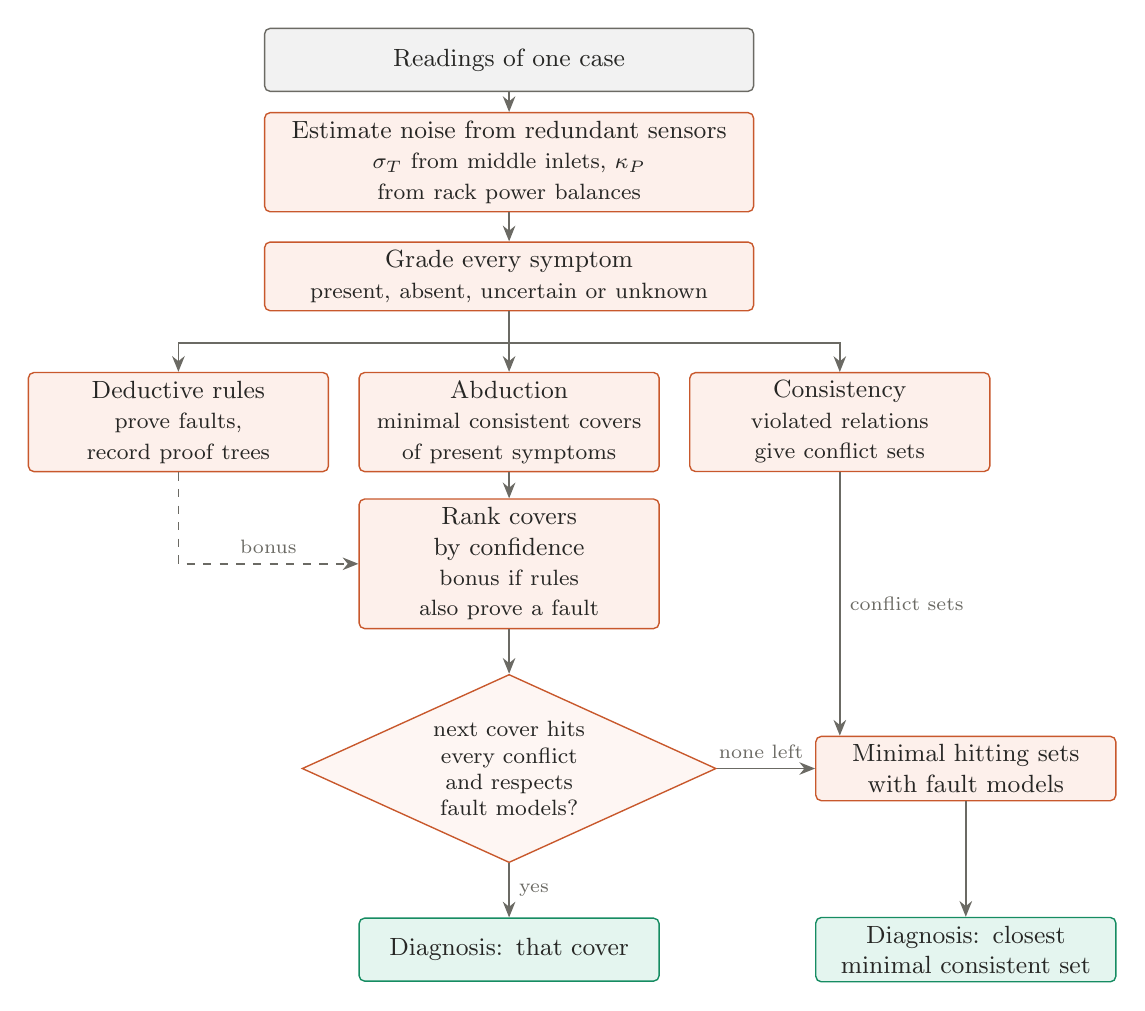
\begin{tikzpicture}[x=1cm, y=1cm]
  \node[data=6cm] (obs) at (4.5,0) {Readings of one case};
  \node[reason=6cm] (noise) at (4.5,-1.3) {Estimate noise from redundant sensors\\ \footnotesize $\sigma_T$ from middle inlets, $\kappa_P$ from rack power balances};
  \node[reason=6cm] (grade) at (4.5,-2.75) {Grade every symptom\\ \footnotesize present, absent, uncertain or unknown};

  \node[reason=3.6cm] (ded) at (0.3,-4.6) {Deductive rules\\ \footnotesize prove faults, record proof trees};
  \node[reason=3.6cm] (abd) at (4.5,-4.6) {Abduction\\ \footnotesize minimal consistent covers of present symptoms};
  \node[reason=3.6cm] (cbd) at (8.7,-4.6) {Consistency\\ \footnotesize violated relations give conflict sets};

  \node[reason=3.6cm] (rank) at (4.5,-6.4) {Rank covers by confidence\\ \footnotesize bonus if rules also prove a fault};
  \node[decision=2.4cm] (dec) at (4.5,-9.0) {next cover hits every conflict and respects fault models?};
  \node[reason=3.6cm] (mhs) at (10.3,-9.0) {Minimal hitting sets with fault models};
  \node[out=3.6cm] (yes) at (4.5,-11.3) {Diagnosis: that cover};
  \node[out=3.6cm] (no) at (10.3,-11.3) {Diagnosis: closest minimal consistent set};

  \draw[flow] (obs) -- (noise);
  \draw[flow] (noise) -- (grade);
  \draw[flow] (grade.south) -- ++(0,-0.4) -| (ded.north);
  \draw[flow] (grade) -- (abd);
  \draw[flow] (grade.south) -- ++(0,-0.4) -| (cbd.north);
  \draw[flow] (abd) -- (rank);
  \draw[uses] (ded.south) |- node[tag, pos=0.75, above] {bonus} (rank.west);
  \draw[flow] (rank) -- (dec);
  \draw[flow] (dec) -- node[tag, right] {yes} (yes);
  \draw[flow] (dec) -- node[tag, above, pos=0.45] {none left} (mhs);
  \draw[flow] (cbd.south) -- node[tag, right] {conflict sets} (cbd.south |- mhs.north);
  \draw[flow] (mhs) -- (no);
\end{tikzpicture}

\end{center}
\clearpage
\section*{fig\_explanation\_workflow}
\begin{center}
% Figure 6: explanation-generation workflow of why/1.
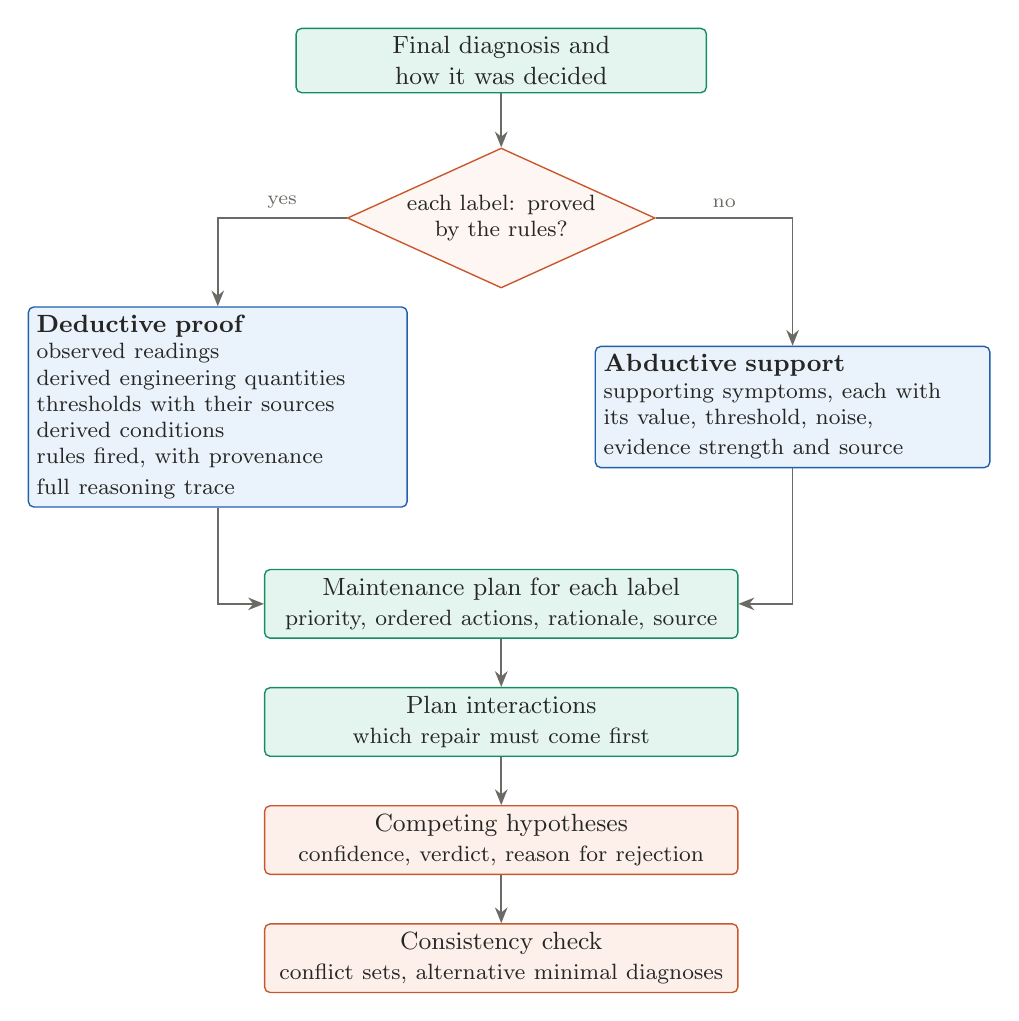
\begin{tikzpicture}[x=1cm, y=1cm]
  \node[out=5cm] (diag) at (4.5,0) {Final diagnosis and how it was decided};
  \node[decision=2.4cm] (dec) at (4.5,-2.0) {each label: proved by the rules?};
  \node[kb=4.6cm, align=left] (proof) at (0.9,-4.4)
    {\textbf{Deductive proof}\\
     \footnotesize observed readings\\
     \footnotesize derived engineering quantities\\
     \footnotesize thresholds with their sources\\
     \footnotesize derived conditions\\
     \footnotesize rules fired, with provenance\\
     \footnotesize full reasoning trace};
  \node[kb=4.8cm, align=left] (abd) at (8.2,-4.4)
    {\textbf{Abductive support}\\
     \footnotesize supporting symptoms, each with\\
     \footnotesize its value, threshold, noise,\\
     \footnotesize evidence strength and source};
  \node[out=5.8cm] (plan) at (4.5,-6.9) {Maintenance plan for each label\\ \footnotesize priority, ordered actions, rationale, source};
  \node[out=5.8cm] (inter) at (4.5,-8.4) {Plan interactions\\ \footnotesize which repair must come first};
  \node[reason=5.8cm] (comp) at (4.5,-9.9) {Competing hypotheses\\ \footnotesize confidence, verdict, reason for rejection};
  \node[reason=5.8cm] (cons) at (4.5,-11.4) {Consistency check\\ \footnotesize conflict sets, alternative minimal diagnoses};

  \draw[flow] (diag) -- (dec);
  \draw[flow] (dec.west) -| node[tag, pos=0.25, above] {yes} (proof.north);
  \draw[flow] (dec.east) -| node[tag, pos=0.25, above] {no} (abd.north);
  \draw[flow] (proof.south) |- (plan.west);
  \draw[flow] (abd.south) |- (plan.east);
  \draw[flow] (plan) -- (inter);
  \draw[flow] (inter) -- (comp);
  \draw[flow] (comp) -- (cons);
\end{tikzpicture}

\end{center}
\clearpage
\section*{fig\_maintenance\_workflow}
\begin{center}
% Figure 7: corrective-maintenance planning workflow.
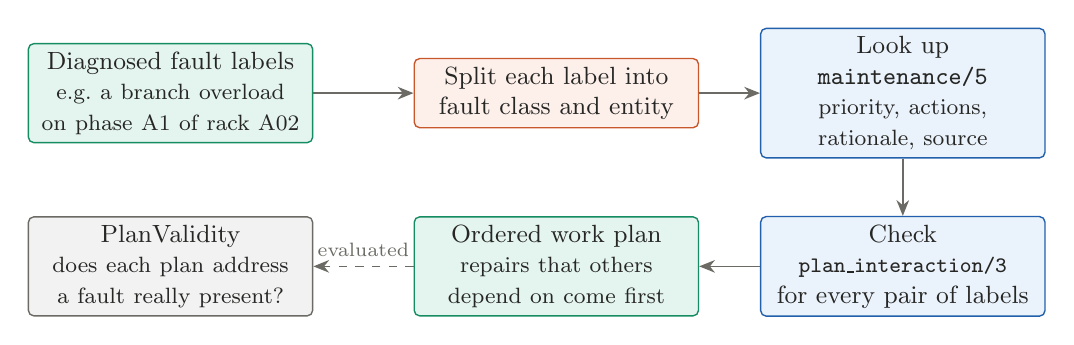
\begin{tikzpicture}[x=1cm, y=1cm]
  \node[out=3.4cm] (lab) at (-0.5,0) {Diagnosed fault labels\\ \footnotesize e.g.\ a branch overload on phase A1 of rack A02};
  \node[reason=3.4cm] (map) at (4.4,0) {Split each label into fault class and entity};
  \node[kb=3.4cm] (kb) at (8.8,0) {Look up \texttt{maintenance/5}\\ \footnotesize priority, actions, rationale, source};
  \node[kb=3.4cm] (int) at (8.8,-2.2) {Check \texttt{\footnotesize plan\_interaction/3} for every pair of labels};
  \node[out=3.4cm] (plan) at (4.4,-2.2) {Ordered work plan\\ \footnotesize repairs that others depend on come first};
  \node[data=3.4cm] (eval) at (-0.5,-2.2) {PlanValidity\\ \footnotesize does each plan address a fault really present?};

  \draw[flow] (lab) -- (map);
  \draw[flow] (map) -- (kb);
  \draw[flow] (kb) -- (int);
  \draw[flow] (int) -- (plan);
  \draw[uses] (plan) -- node[tag, above] {evaluated} (eval);
\end{tikzpicture}

\end{center}
\clearpage
\section*{fig\_evaluation\_workflow}
\begin{center}
% Figure 8: experimental and evaluation workflow.
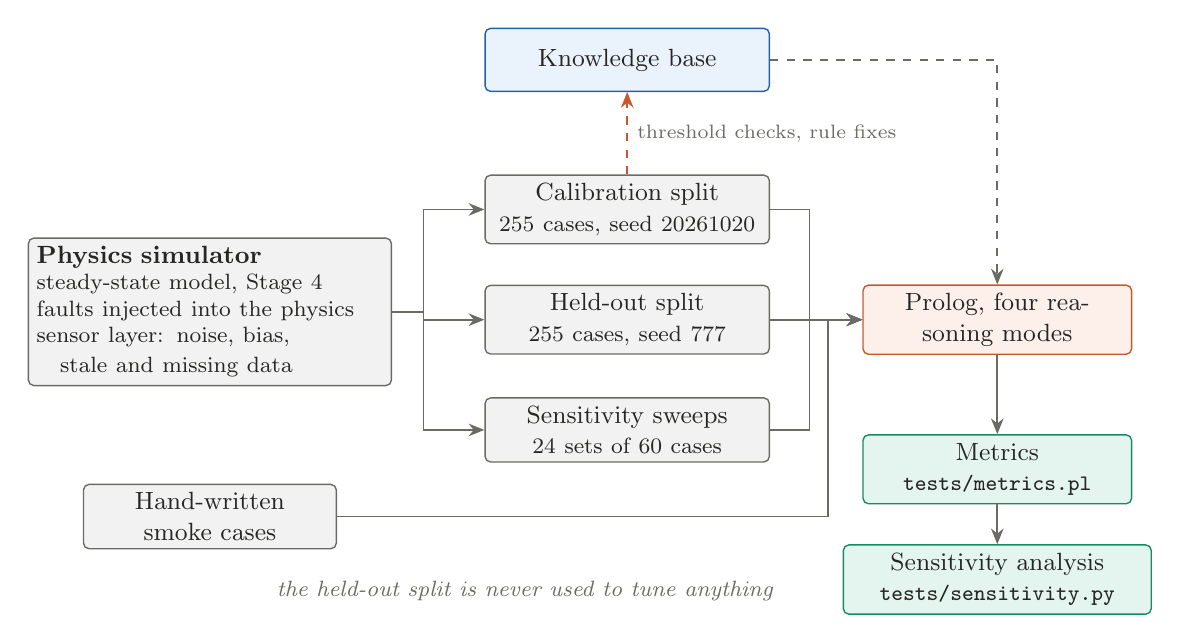
\begin{tikzpicture}[x=1cm, y=1cm]
  \node[data=4.4cm, align=left] (sim) at (0.6,0)
    {\textbf{Physics simulator}\\
     \footnotesize steady-state model, Stage 4\\
     \footnotesize faults injected into the physics\\
     \footnotesize sensor layer: noise, bias,\\
     \footnotesize \quad stale and missing data};
  \node[data=3cm] (hand) at (0.6,-2.6) {Hand-written smoke cases};

  \node[data=3.4cm] (cal) at (5.9,1.3) {Calibration split\\ \footnotesize 255 cases, seed 20261020};
  \node[data=3.4cm] (hold) at (5.9,-0.1) {Held-out split\\ \footnotesize 255 cases, seed 777};
  \node[data=3.4cm] (swp) at (5.9,-1.5) {Sensitivity sweeps\\ \footnotesize 24 sets of 60 cases};

  \node[reason=3.2cm] (pl) at (10.6,-0.1) {Prolog, four reasoning modes};
  \node[out=3.2cm] (met) at (10.6,-2.0) {Metrics\\ \footnotesize \texttt{tests/metrics.pl}};
  \node[out=3.7cm] (sen) at (10.6,-3.4) {Sensitivity analysis\\ \footnotesize \texttt{tests/sensitivity.py}};
  \node[kb=3.4cm] (kb) at (5.9,3.2) {Knowledge base};

  \draw[flow] (sim.east) -- ++(0.4,0) |- (cal.west);
  \draw[flow] (sim.east) -- ++(0.4,0) |- (hold.west);
  \draw[flow] (sim.east) -- ++(0.4,0) |- (swp.west);
  \draw[flow] (hand.east) -- (8.45,-2.6) |- (pl.west);
  \draw[flow] (cal.east) -- ++(0.5,0) |- (pl.west);
  \draw[flow] (hold) -- (pl);
  \draw[flow] (swp.east) -- ++(0.5,0) |- (pl.west);
  \draw[flow] (pl) -- (met);
  \draw[flow] (met) -- (sen);
  \draw[uses] (kb.east) -| (pl.north);
  \draw[feedback] (cal.north) -- node[tag, right] {threshold checks, rule fixes} (kb.south);
  \node[note] at (4.6,-3.55) {the held-out split is never used to tune anything};
\end{tikzpicture}

\end{center}
\clearpage
\section*{sens\_noise}
\begin{center}
% Generated by tests/sensitivity.py. Do not edit by hand.
% Needs \usepackage{pgfplots} and \pgfplotsset{compat=1.18} in the preamble.
% Colours: validated categorical palette, slots 1 to 4. Marker and dash repeat the identity.
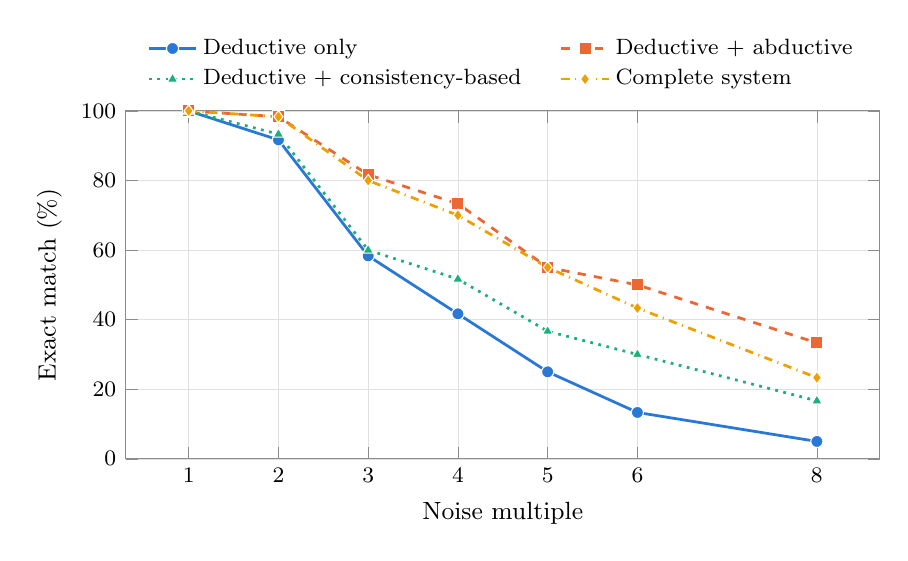
\begin{tikzpicture}
\definecolor{modedeductive}{HTML}{2a78d6}
\definecolor{modededabd}{HTML}{eb6834}
\definecolor{modededcbd}{HTML}{1baf7a}
\definecolor{modefull}{HTML}{eda100}
\begin{axis}[
  width=0.92\linewidth, height=6cm,
  xlabel={Noise multiple}, ylabel={Exact match (\%)},
  ymin=0, ymax=100,
  xtick={1,2,3,4,5,6,8},
  grid=major, major grid style={line width=0.2pt, draw=black!12},
  axis line style={draw=black!45}, tick style={draw=black!45},
  label style={font=\small}, tick label style={font=\footnotesize},
  legend style={font=\footnotesize, draw=none, fill=none, at={(0.5,1.03)}, anchor=south, legend columns=2,
    /tikz/every even column/.append style={column sep=1.2em}},
  legend cell align=left,
]
\addplot[color=modedeductive, solid, line width=1pt, mark=*, mark size=2.2pt, mark options={solid, draw=white, line width=0.4pt}] coordinates {(1,100.00) (2,91.67) (3,58.33) (4,41.67) (5,25.00) (6,13.33) (8,5.00)};
\addlegendentry{Deductive only}
\addplot[color=modededabd, dashed, line width=1pt, mark=square*, mark size=2.2pt, mark options={solid, draw=white, line width=0.4pt}] coordinates {(1,100.00) (2,98.33) (3,81.67) (4,73.33) (5,55.00) (6,50.00) (8,33.33)};
\addlegendentry{Deductive + abductive}
\addplot[color=modededcbd, dotted, line width=1pt, mark=triangle*, mark size=2.2pt, mark options={solid, draw=white, line width=0.4pt}] coordinates {(1,100.00) (2,93.33) (3,60.00) (4,51.67) (5,36.67) (6,30.00) (8,16.67)};
\addlegendentry{Deductive + consistency-based}
\addplot[color=modefull, dashdotted, line width=1pt, mark=diamond*, mark size=2.2pt, mark options={solid, draw=white, line width=0.4pt}] coordinates {(1,100.00) (2,98.33) (3,80.00) (4,70.00) (5,55.00) (6,43.33) (8,23.33)};
\addlegendentry{Complete system}
\end{axis}
\end{tikzpicture}

\end{center}
\clearpage
\section*{sens\_missing}
\begin{center}
% Generated by tests/sensitivity.py. Do not edit by hand.
% Needs \usepackage{pgfplots} and \pgfplotsset{compat=1.18} in the preamble.
% Colours: validated categorical palette, slots 1 to 4. Marker and dash repeat the identity.
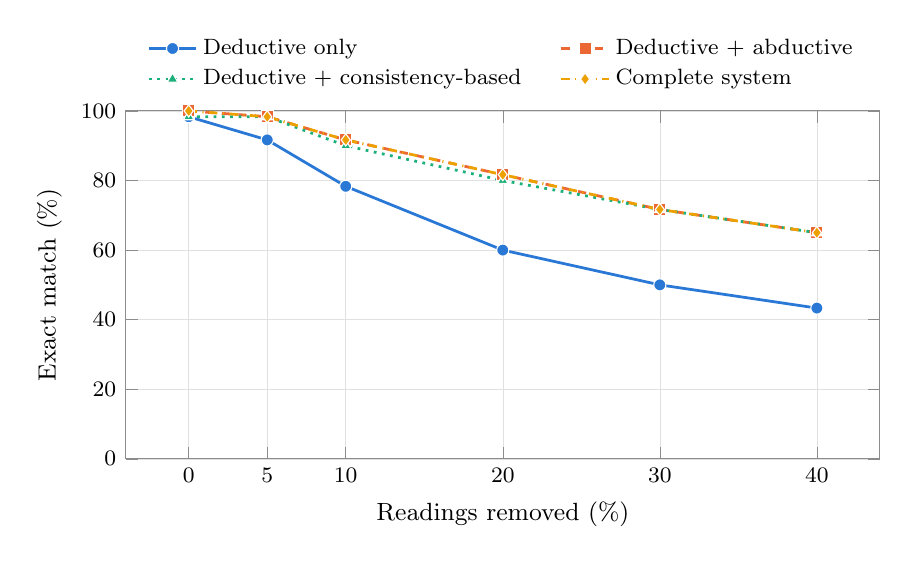
\begin{tikzpicture}
\definecolor{modedeductive}{HTML}{2a78d6}
\definecolor{modededabd}{HTML}{eb6834}
\definecolor{modededcbd}{HTML}{1baf7a}
\definecolor{modefull}{HTML}{eda100}
\begin{axis}[
  width=0.92\linewidth, height=6cm,
  xlabel={Readings removed (\%)}, ylabel={Exact match (\%)},
  ymin=0, ymax=100,
  xtick={0,5,10,20,30,40},
  grid=major, major grid style={line width=0.2pt, draw=black!12},
  axis line style={draw=black!45}, tick style={draw=black!45},
  label style={font=\small}, tick label style={font=\footnotesize},
  legend style={font=\footnotesize, draw=none, fill=none, at={(0.5,1.03)}, anchor=south, legend columns=2,
    /tikz/every even column/.append style={column sep=1.2em}},
  legend cell align=left,
]
\addplot[color=modedeductive, solid, line width=1pt, mark=*, mark size=2.2pt, mark options={solid, draw=white, line width=0.4pt}] coordinates {(0,98.33) (5,91.67) (10,78.33) (20,60.00) (30,50.00) (40,43.33)};
\addlegendentry{Deductive only}
\addplot[color=modededabd, dashed, line width=1pt, mark=square*, mark size=2.2pt, mark options={solid, draw=white, line width=0.4pt}] coordinates {(0,100.00) (5,98.33) (10,91.67) (20,81.67) (30,71.67) (40,65.00)};
\addlegendentry{Deductive + abductive}
\addplot[color=modededcbd, dotted, line width=1pt, mark=triangle*, mark size=2.2pt, mark options={solid, draw=white, line width=0.4pt}] coordinates {(0,98.33) (5,98.33) (10,90.00) (20,80.00) (30,71.67) (40,65.00)};
\addlegendentry{Deductive + consistency-based}
\addplot[color=modefull, dashdotted, line width=1pt, mark=diamond*, mark size=2.2pt, mark options={solid, draw=white, line width=0.4pt}] coordinates {(0,100.00) (5,98.33) (10,91.67) (20,81.67) (30,71.67) (40,65.00)};
\addlegendentry{Complete system}
\end{axis}
\end{tikzpicture}

\end{center}
\clearpage
\section*{sens\_multi}
\begin{center}
% Generated by tests/sensitivity.py. Do not edit by hand.
% Needs \usepackage{pgfplots} and \pgfplotsset{compat=1.18} in the preamble.
% Colours: validated categorical palette, slots 1 to 4. Marker and dash repeat the identity.
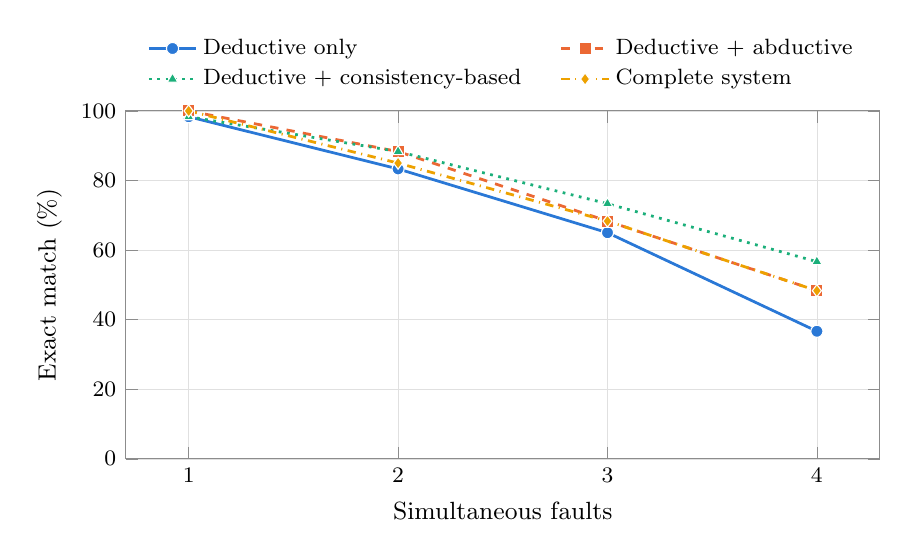
\begin{tikzpicture}
\definecolor{modedeductive}{HTML}{2a78d6}
\definecolor{modededabd}{HTML}{eb6834}
\definecolor{modededcbd}{HTML}{1baf7a}
\definecolor{modefull}{HTML}{eda100}
\begin{axis}[
  width=0.92\linewidth, height=6cm,
  xlabel={Simultaneous faults}, ylabel={Exact match (\%)},
  ymin=0, ymax=100,
  xtick={1,2,3,4},
  grid=major, major grid style={line width=0.2pt, draw=black!12},
  axis line style={draw=black!45}, tick style={draw=black!45},
  label style={font=\small}, tick label style={font=\footnotesize},
  legend style={font=\footnotesize, draw=none, fill=none, at={(0.5,1.03)}, anchor=south, legend columns=2,
    /tikz/every even column/.append style={column sep=1.2em}},
  legend cell align=left,
]
\addplot[color=modedeductive, solid, line width=1pt, mark=*, mark size=2.2pt, mark options={solid, draw=white, line width=0.4pt}] coordinates {(1,98.33) (2,83.33) (3,65.00) (4,36.67)};
\addlegendentry{Deductive only}
\addplot[color=modededabd, dashed, line width=1pt, mark=square*, mark size=2.2pt, mark options={solid, draw=white, line width=0.4pt}] coordinates {(1,100.00) (2,88.33) (3,68.33) (4,48.33)};
\addlegendentry{Deductive + abductive}
\addplot[color=modededcbd, dotted, line width=1pt, mark=triangle*, mark size=2.2pt, mark options={solid, draw=white, line width=0.4pt}] coordinates {(1,98.33) (2,88.33) (3,73.33) (4,56.67)};
\addlegendentry{Deductive + consistency-based}
\addplot[color=modefull, dashdotted, line width=1pt, mark=diamond*, mark size=2.2pt, mark options={solid, draw=white, line width=0.4pt}] coordinates {(1,100.00) (2,85.00) (3,68.33) (4,48.33)};
\addlegendentry{Complete system}
\end{axis}
\end{tikzpicture}

\end{center}
\clearpage
\section*{sens\_multi\_time}
\begin{center}
% Generated by tests/sensitivity.py. Do not edit by hand.
% Needs \usepackage{pgfplots} and \pgfplotsset{compat=1.18} in the preamble.
% Colours: validated categorical palette, slots 1 to 4. Marker and dash repeat the identity.
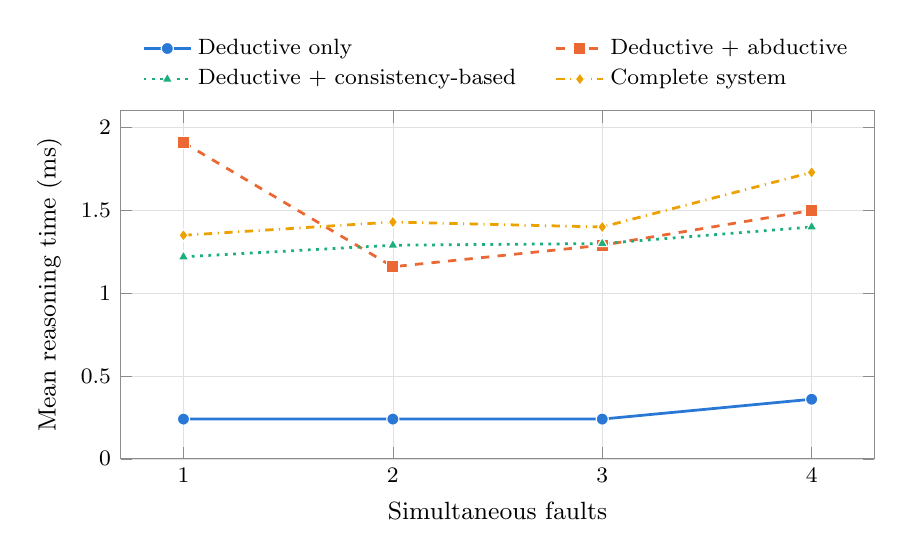
\begin{tikzpicture}
\definecolor{modedeductive}{HTML}{2a78d6}
\definecolor{modededabd}{HTML}{eb6834}
\definecolor{modededcbd}{HTML}{1baf7a}
\definecolor{modefull}{HTML}{eda100}
\begin{axis}[
  width=0.92\linewidth, height=6cm,
  xlabel={Simultaneous faults}, ylabel={Mean reasoning time (ms)},
  ymin=0,
  xtick={1,2,3,4},
  grid=major, major grid style={line width=0.2pt, draw=black!12},
  axis line style={draw=black!45}, tick style={draw=black!45},
  label style={font=\small}, tick label style={font=\footnotesize},
  legend style={font=\footnotesize, draw=none, fill=none, at={(0.5,1.03)}, anchor=south, legend columns=2,
    /tikz/every even column/.append style={column sep=1.2em}},
  legend cell align=left,
]
\addplot[color=modedeductive, solid, line width=1pt, mark=*, mark size=2.2pt, mark options={solid, draw=white, line width=0.4pt}] coordinates {(1,0.24) (2,0.24) (3,0.24) (4,0.36)};
\addlegendentry{Deductive only}
\addplot[color=modededabd, dashed, line width=1pt, mark=square*, mark size=2.2pt, mark options={solid, draw=white, line width=0.4pt}] coordinates {(1,1.91) (2,1.16) (3,1.29) (4,1.50)};
\addlegendentry{Deductive + abductive}
\addplot[color=modededcbd, dotted, line width=1pt, mark=triangle*, mark size=2.2pt, mark options={solid, draw=white, line width=0.4pt}] coordinates {(1,1.22) (2,1.29) (3,1.30) (4,1.40)};
\addlegendentry{Deductive + consistency-based}
\addplot[color=modefull, dashdotted, line width=1pt, mark=diamond*, mark size=2.2pt, mark options={solid, draw=white, line width=0.4pt}] coordinates {(1,1.35) (2,1.43) (3,1.40) (4,1.73)};
\addlegendentry{Complete system}
\end{axis}
\end{tikzpicture}

\end{center}
\clearpage
\section*{sens\_bias}
\begin{center}
% Generated by tests/sensitivity.py. Do not edit by hand.
% Needs \usepackage{pgfplots} and \pgfplotsset{compat=1.18} in the preamble.
% Colours: validated categorical palette, slots 1 to 4. Marker and dash repeat the identity.
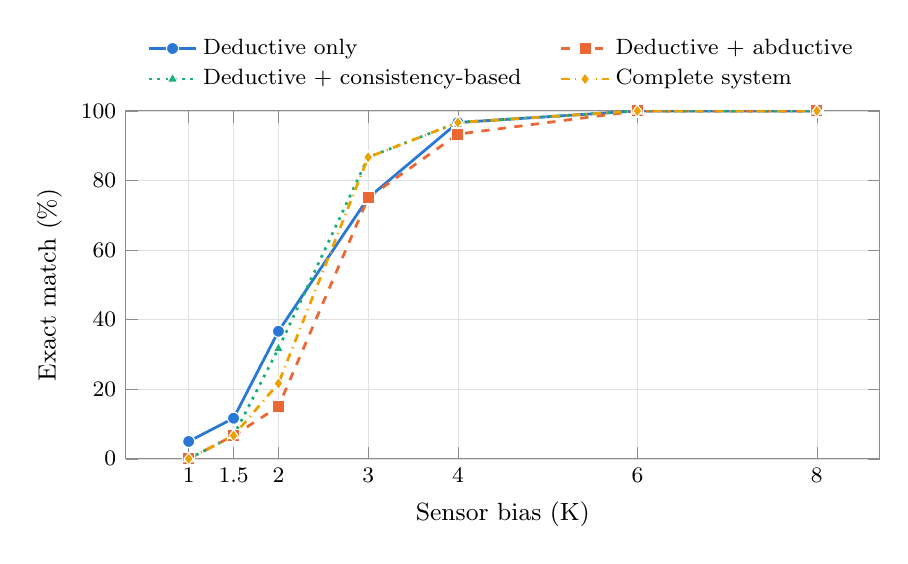
\begin{tikzpicture}
\definecolor{modedeductive}{HTML}{2a78d6}
\definecolor{modededabd}{HTML}{eb6834}
\definecolor{modededcbd}{HTML}{1baf7a}
\definecolor{modefull}{HTML}{eda100}
\begin{axis}[
  width=0.92\linewidth, height=6cm,
  xlabel={Sensor bias (K)}, ylabel={Exact match (\%)},
  ymin=0, ymax=100,
  xtick={1,1.5,2,3,4,6,8},
  grid=major, major grid style={line width=0.2pt, draw=black!12},
  axis line style={draw=black!45}, tick style={draw=black!45},
  label style={font=\small}, tick label style={font=\footnotesize},
  legend style={font=\footnotesize, draw=none, fill=none, at={(0.5,1.03)}, anchor=south, legend columns=2,
    /tikz/every even column/.append style={column sep=1.2em}},
  legend cell align=left,
]
\addplot[color=modedeductive, solid, line width=1pt, mark=*, mark size=2.2pt, mark options={solid, draw=white, line width=0.4pt}] coordinates {(1,5.00) (1.5,11.67) (2,36.67) (3,75.00) (4,96.67) (6,100.00) (8,100.00)};
\addlegendentry{Deductive only}
\addplot[color=modededabd, dashed, line width=1pt, mark=square*, mark size=2.2pt, mark options={solid, draw=white, line width=0.4pt}] coordinates {(1,0.00) (1.5,6.67) (2,15.00) (3,75.00) (4,93.33) (6,100.00) (8,100.00)};
\addlegendentry{Deductive + abductive}
\addplot[color=modededcbd, dotted, line width=1pt, mark=triangle*, mark size=2.2pt, mark options={solid, draw=white, line width=0.4pt}] coordinates {(1,0.00) (1.5,6.67) (2,31.67) (3,86.67) (4,96.67) (6,100.00) (8,100.00)};
\addlegendentry{Deductive + consistency-based}
\addplot[color=modefull, dashdotted, line width=1pt, mark=diamond*, mark size=2.2pt, mark options={solid, draw=white, line width=0.4pt}] coordinates {(1,0.00) (1.5,6.67) (2,21.67) (3,86.67) (4,96.67) (6,100.00) (8,100.00)};
\addlegendentry{Complete system}
\end{axis}
\end{tikzpicture}

\end{center}
\clearpage
\end{document}
